\documentclass[bibliography=totoc]{article}
\usepackage{titling}
\usepackage{listings}
%\usepackage[nottoc,numbib]{tocbibind}
\usepackage[nottoc]{tocbibind}

%\documentclass[bibliography=totoc]{scrartcl}

\usepackage[lithuanian]{babel}
\usepackage[utf8x]{inputenc}
\def\LTfontencoding{L7x}
%\PrerenderUnicode{ąčęėįšųūž}
\usepackage[\LTfontencoding]{fontenc}
\usepackage[T1]{fontenc}


\usepackage{geometry}
 \geometry{
 a4paper,
 total={170mm,257mm},
 left=20mm,
 top=20mm,
 }

\usepackage{natbib}
\usepackage{amssymb}
\usepackage{amsmath}
\usepackage{multicol}
\usepackage{tikz}
\usetikzlibrary{arrows, automata}
\usepackage{algorithm}
\usepackage{algorithmic}
\usepackage{wrapfig}
\usepackage{graphicx}
\usepackage{float}
\usepackage{caption}
\usepackage{subcaption}
\usepackage{hyperref}
\newtheorem{definition}{Apibrėžimas}
\newtheorem{example}{Pavyzdys}
\newtheorem{experiment}{Grafas}

\begin{document}

\begin{titlepage}
    \begin{center}
        \vspace*{1cm}
 
        \Huge
        \textbf{Vilniaus Universitetas}\\
         \textbf{Informatikos institutas}\\
        
        \vspace{6.5cm}
        \textbf{Vasarė Pratuzaite ir Akvilė Ropytė}\\
       \textit{ informatikos specialybė, \\
                 II kursas, 1, 3 grupės\\}
        \textbf{Skirtumo paieška tarp ilgiausio ir trumpiausio kelio grafe, gauto, naudojant Floyd-Warshall algoritmą}\\
          
                 
 
        \vfill
        Vilnius -- 2024
    \end{center}
\end{titlepage}
\tableofcontents
\newpage
\section*{Įvadas}
\label{sec:ivadas}
\addcontentsline{toc}{section}{\nameref{sec:ivadas}}

Saugumas ir greitis yra vienas iš svarbiausių algoritmų savybių, todėl šios ypatybės padaro algoritmą optimalų.

Prieš daugiau nei keturius dešimtmečius, kai amerikiečių kompiuterių mokslininkas Stephen‘as Warshall'as (1959) ir  Robert‘as Floyd'as(1962) paskelbė savo plačiai naudojamus algoritmus, skirtus aptikti bet kokias kilpas arba apskaičiuoti visas poras trumpiausių kelių orientuotame, svoriniame grafe, įvyko reikšmingas proveržis grafų teorijoje. Jo indėlis apima Floydo-Warshall algoritmo (nepriklausomai nuo Stepheno Warshallo), kuris efektyviai randa visus trumpiausius kelius tarp grafo viršūnių, sukūrimą ir jo darbą analizuojant.

Pagrindinė algoritmo idėja yra triviali: jei egzistuoja keliai P[i,k] ir P[k,j], tai egzistuoja ir kelias P[i,j]. Tai leidžia atlikti visų porų analizę ir gauti įvairiapusę informaciją apie grafo struktūrą, sistemiškai sekant veikimo (kaimynystės) informacinę sistemą mazgas po mazgo (k) per grafą.

Šiame darbe tiriami grafai, naudojant Floyd-Warshall algoritmą, kuris skirtas apskaičiuoti trumpiausius kelius tarp visų porų viršūnių orientuotuose, svoriu paženklintuose grafuose. Grafų teorija ir algoritmai yra esminiai įrankiai kompiuterių mokslo ir matematikos srityse, turintys platų pritaikymą nuo transporto tinklų optimizavimo iki socialinių tinklų analizės.

Tyrimo tikslas yra analizuoti, pritaikius Floyd-Warshall algoritmą, gautų trumpiausių atstumų skirtumą - skirtumą tarp ilgiausio ir trumpiausio kelio. Taip pat išsiaiškinti, kokią informaciją apie grafo struktūrą galima gauti iš šios analizės. Šiame tyrime bus nagrinėjama, kaip kinta minėtas skirtumas skirtingų struktūrų grafuose.



Iškelta hipotezė - kuo daugiau kaimynių turi grafo viršūnės, tuo skirtumas tarp ilgiausio ir trumpiausio kelio bus mažesnis.

Tyrimui naudojami 2 skirtingi orientuoti svoriniai grafai, turintys po 10 viršūnių, kur kiekviena viršūnė turi 3 kaimynus viename grafe ir 4 kitame. Tyrimą sudaro šie etapai:
\begin{enumerate}
    \item Grafų generavimas pagal nurodytas struktūrines savybes.
    \item Floyd-Warshall algoritmo pritaikymas šiems grafams.
    \item Gautų skirtumų tarp ilgiausio ir trumpiausio atstumo analizavimas.    
\end{enumerate}


%%%%%%%%%%%%%%%%%%%%%%%%%%%%%%%%%%%%%%%%%%%%%%%%%%%%%%%%%%%%%%%%%%%%%%%%%
\newpage
\section{Apibrėžimai. Tiriamoji grafų klasė}

\begin{definition}[Orientuotas grafas]
    Grafas $G = (V, E)$, kuriame $V$ yra viršūnių aibė ir $E$ yra briaunų aibė, yra orientuotas, jei kiekviena briauna turi priskirtą kryptį.
\end{definition}

\begin{definition}[Svorinis grafas]
Tai toks grafas $G=(V, E)$, kuriame kiekvienai briaunai $e \in E$ yra priskritas svoris - skaičius, kuris paprastai žymimas $w(e)$. Formaliu būdu, svorinį grafą galima apibrėžti kaip grafą $G = (V, E, w)$, kur $w: E \rightarrow \mathbb{R}^{+}$ yra funkcija, kuri kiekvienai briaunai $e \in E$ priskiria teigiamą realųjį skaičių.
\end{definition}


\begin{definition}[Grafo uždarinys]
    Grafo $G$ uždarinys yra grafas $G^*$, gautas iš grafo $G$, vis pridedant kraštines tarp neincidenčių viršūnių, kurių laipsnių suma yra nemažesnė nei grafo $G$ viršūnių skaičius.
\end{definition}


\begin{definition}[Tranzityvumas]
Tranzityvumas – tai sąryšio $R$ tarp dviejų aibės elementų apibūdinimas. Tarkime, turime aibę $X$, kurioje yra elementai $\{x, y, z\}$. Jei aibės elementų pora $(x, y)$ tenkina sąryšį $(x \, R \, y)$ ir pora $(y, z)$ tenkina sąryšį $(y \, R \, z)$, tai sąryšis yra tranzityvus, jei $(x \, R \, z)$ galioja ir porai $(x, z)$ (kiekvienam $x, y, z$ iš aibės $X$). 
\end{definition}



\begin{definition}[Tranzityvus grafas]
    Tai toks grafas $G = (V, E)$, kurio viršūnių poroms $(a, b)$ ir $(b, c)$ egzistuoja viršūnių pora $(a, c)$. T.y., jei iš $a$ galime nueiti į $b$ ir iš $b$ nueiti į $c$, tai tada iš $a$ galime nueiti į $c$.
\end{definition}

\begin{definition}[Tranzityvus grafo uždarinys]
    Tai duomenų struktūra, kurioje pavaizduoti visi galimiausi keliai tarp kiekvienos viršūnės. Kitaip, iš grafo $G = (V, E)$ gauname tranzityvų grafo uždarinį $G^* = (V, E)$, kur yra briauna $(u, v)$, priklausanti aibei $E^*$, jei grafe $G$ yra kelias iš $u$ į $v$.
\end{definition}

\begin{definition}[Trumpiausias kelias tarp dviejų viršūnių]
Trumpiausias kelias tarp dviejų viršūnių $u$ ir $v$ svoriniame orientuotame grafe $G=(V, E)$ yra tokia viršūnių seka, kad briaunų svoriai būtų mažiausi tarp visų galimų kelių iš viršūnės $u$ į viršūnę $v$.
\end{definition}

\begin{definition}[Floyd-Warshall algoritmas]
    Šis algoritmas naudojamas rasti trumpiausius kelius tarp visų porų viršūnių svoriniuose grafuose. Šis algoritmas tinka tiek orientuotiems, tiek neorientuotiems grafams ir gali tvarkyti neigiamus briaunų svorius, jei nėra neigiamų ciklų.
\end{definition}











%%%%%%%%%%%%%%%%%%%%%%%%%%%%%%%%%%%%%%%%%%%%%%%%%%%%%%%%%%%%%%%%%%%%%%%%%
\newpage
\section{Algoritmai}

\begin{algorithm}[h]
    \caption{Floyd-Warshall algoritmas}
    \textbf{Duota:} Orientuotas svorinis grafas $G=(V,E)$\\
    \textbf{Rasti:} Trumpiausius kelius tarp kiekvienos viršūnės\\
    \textbf{floyd\_warshall} $(G)$ (iš Networkx bibliotekos)
\end{algorithm}

 Dabar žinomas algoritmas buvo paskelbtas Roberto Floido (angl. Robert Floyd) 1962 m. Tačiau šis algoritmas buvo labai panašus į anksčiau išleistą Stefano Varšalo (angl. Stephen Warshall) algoritmą tranzityvaus grafo uždariniui rasti.
 Floyd-Warshall algoritmas skirtas rasti trumpiausius kelius tarp kiekvienos viršūnės orientuotame svoriniame grafe. Algoritmas sukonstruoja naują svorinį grafą iš  duoto svorinio grafo, kuriame kiekvienai briaunai pateikiamas svoris, atitinkantis minimaliam svoriui kažkokio kelio tarp tos briaunos viršūnių. Algoritmas tinka ir grafui, kurio briaunų svoriai yra neigiami, tačiau, jei grafe bus neigiamų ciklų, tai algoritmas neveiks korektiškai.

\begin{algorithm}[h]
    \caption{Grafo su k kaimynų generavimo algoritmas}
    \textbf{Duota:} Viršūnių skaičius $n$, kaimynų skaičius $k$, minimalus atstumas $min\_distance$, maksimalus atstumas $max\_distance$\\
    \textbf{Rasti:} Sugeneruotą orientuotą svorinį grafą $G=(V, E)$
    \begin{algorithmic}[1]
        \STATE $G \gets$ tuščias grafas
        \FOR{$node$ \textbf{from} $1$ \textbf{to} $n$}
            \STATE $G$.add\_node($node$)
        \ENDFOR
        \FOR{$node$ \textbf{from} $1$ \textbf{to} $n$}
            \STATE $candidate\_nodes \gets$ sąrašas visų viršūnių, išskyrus $node$, kurios turi mažiau nei $k$ kaimynų
            \STATE $neighbors \gets$ atsitiktinai pasirinkti $min(k, (candidate\_nodes))$ kaimynai iš $candidate\_nodes$
            \FOR{$neighbor$ \textbf{in} $neighbors$}
                \STATE $weight \gets$ atsitiktinis svoris intervale nuo $min\_distance$ iki $max\_distance$
                \STATE $G$.add\_edge($node$, $neighbor$, weight=$weight$)
            \ENDFOR
        \ENDFOR
        \RETURN $G$
    \end{algorithmic}
\end{algorithm}


\begin{algorithm}[h]
    \caption{Trumpiausių kelių skirtumo tarp ilgiausio ir trumpiausio kelių algortimas }
    \textbf{Duota:} Orientuotas svorinis grafas $G=(V,E)$\\
    \textbf{Rasti:} Trumpiausių kelių skirtumas tarp ilgiausio ir trumpiausio kelio
    \begin{algorithmic}[1]
        \STATE $shortest\_paths \gets floyd\_warshall(G)$
        \STATE $max\_shortest\_path \gets -\infty$
        \STATE $min\_shortest\_path \gets +\infty$
        \FOR{$start\_node$ \textbf{in} $shortest\_paths$}
            \FOR{$end\_node$ \textbf{in} $shortest\_paths[start\_node]$}
                \IF{$start\_node \neq end\_node$}
                    \STATE $shortest\_path \gets shortest\_paths[start\_node][end\_node]$
                    \IF{$shortest\_path > max\_shortest\_path$}
                        \STATE $max\_shortest\_path \gets shortest\_path$
                    \ENDIF
                    \IF{$shortest\_path < min\_shortest\_path$}
                        \STATE $min\_shortest\_path \gets shortest\_path$
                    \ENDIF
                \ENDIF
            \ENDFOR
        \ENDFOR
        \RETURN $max\_shortest\_path - min\_shortest\_path$
    \end{algorithmic}
\end{algorithm}

%\clearpage
\newpage
%%%%%%%%%%%%%%%%%%%%%%%%%%%%%%%%%%%%%%%%%%%%%%%%%%%%%%%%%%%%%%%%%%%%%%%%%
\section{Algoritmų realizacija ir tyrimų eiga}
Algoritmas įgyvendintas $Python$ programavimo kalba, naudojantis NetworkX, Pyplot, Random ir Numpy bibliotekomis. Grafui, sugeneruotam pagal grafo su k kaimynėmis algoritmu, buvo pritaikyta Networkx įgvendinta Floyd-Warshall algoritmo funkcija. Random buvo naudojama atsitiktiniam kelio tarp viršūnių ilgiui ir viršūnės kaimynams parinkti. Numpy naudota rasti masyvo vidurkiui, o Pyplot - atvaizduoti gautiems duomenims.\\

\textbf{Algoritmas:}
\begin{enumerate}
    \item Sugeneruojama 10000 grafų ir jiems pritaikomas Floyd-Warshall algoritmas.
    \item Ieškomas skirtumas tarp ilgiausio ir trumpiausio kelio.
    \item Šis procesas kartojamas 200 kartų.
\end{enumerate}

\textbf{Pagrindiniai tyrimo objektai:}
\begin{enumerate}
    \item Ilgiausio ir trumpiausio kelio skirtumas trumpiausių kelių grafe.
    \item Didžiausi skirtumai.
    \item Skirtumo vidurkis.\\
\end{enumerate}

Tyrimai vykdyti pagal skirtingą grafo viršūnių kaimynių skaičių: k = 3 ir k = 4.


\newpage
\section{Tyrimų rezultatai ir jų aptarimas}

Paveikslėliuose \ref{fig:skirtumas_k3} ir \ref{fig:skirtumas_k4} pavaizduoti skirtumai trumpiausių atstumų grafuose, kai kiekviena viršūnė turi atitinkamai 3 ir 4 kaimynus.
Pirmuoju atveju dažniausiai pasikartojantys skirtumai yra 16 ir 17, na o kai kiekvienos viršūnės kaimynių skaičius yra 4, tai dažniausias skirtumas yra 13. Šiek tiek mažiau pasikartoja ir 12 bei 14.
 
Taigi, dažniausiai pasitaikantis skirtumas, kai viršūnės turi po 4 kaimynus, yra 3 vienetais mažesnis, nei grafe, kurio viršūnės turi po 3 kaimynus.



\begin{figure}[h]
\centering
\begin{subfigure}{.5\textwidth}
    \centering
    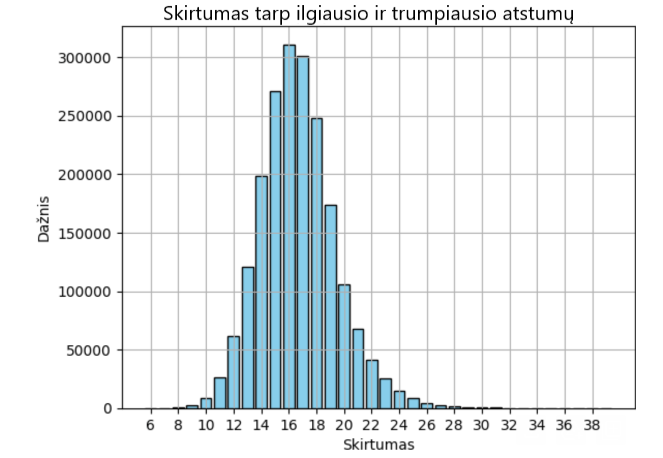
\includegraphics[scale = .5]{skirtumas_k3.png}
    \caption{viršūnės kaimynių skaičius = 3}
    \label{fig:skirtumas_k3}
\end{subfigure}%
\begin{subfigure}{.5\textwidth}
    \centering
    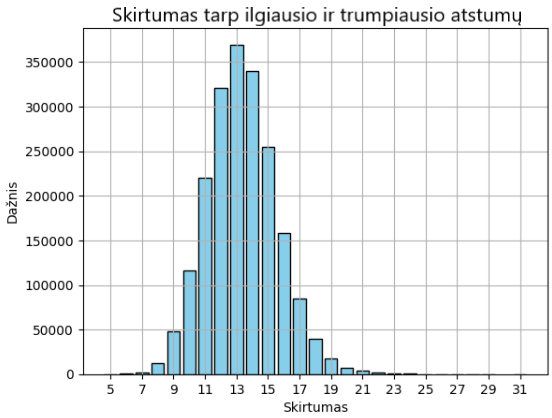
\includegraphics[scale = .55]{skirtumas_k4.png}
    \caption{viršūnės kaimynių skaičius = 4}
    \label{fig:skirtumas_k4}
\end{subfigure}
\caption{}
\end{figure}

Sekančiuose grafikuose matomi didžiausi skirtumai tarp ilgiausių ir trumpiausių kelių grafuose. Kiekviena viršūnė atitinkamai grafuose turi po 3 ir 4 kaimynes. Paveikslėlyje \ref{fig:did_skirtumas_k3}, kai viršūnių skaičius yra trys, nesunku pastebėti, kad labiausiai pasikartojantys didžiausi skirtumai yra 31, 32, bei 33, o gretimoje diagramoje \ref{did_skirtumas_k4} gerokai mažiau – tik 24, 25 bei 26. Taigi, kai grafo viršūnės turi vienetu daugiau kaimynų, tai dažniausiai pasikartojantis didžiausias skirtumas sumažėja per 6 vienetus.

\begin{figure}[h]
\centering
\begin{subfigure}{.5\textwidth}
  \centering
  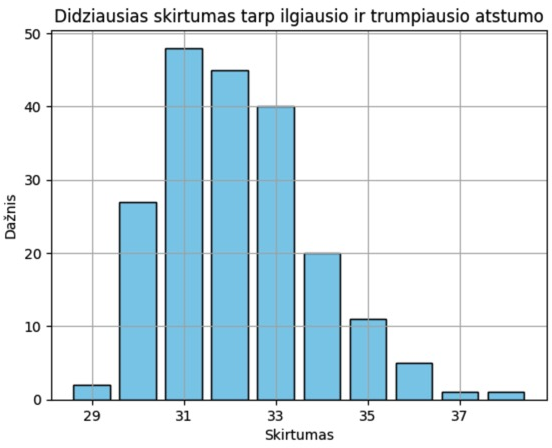
\includegraphics[scale = .52]{didziausias_skirtumas_k3.png}
    \caption{viršūnės kaimynių skaičius = 3}
  \label{fig:did_skirtumas_k3}
\end{subfigure}%
\begin{subfigure}{.5\textwidth}
  \centering
  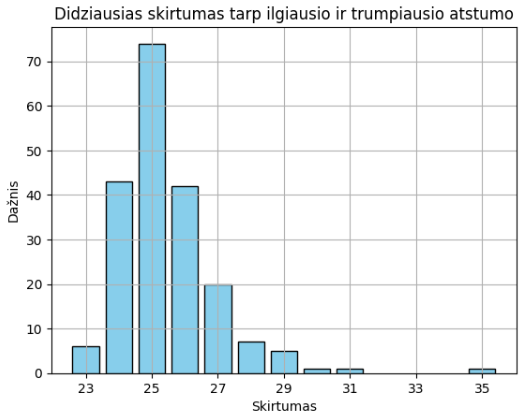
\includegraphics[scale = .7]{didziausias_skirtumas_k4.png}
    \caption{viršūnės kaimynių skaičius = 4}
  \label{did_skirtumas_k4}
\end{subfigure}
\caption{}
\end{figure}
\newpage

Toliau buvo nagrinėjamas gautų skirtumų vidurkis. Iš gautų rezultatų galima pastebėti, kad jis kinta nežymiai. \ref{fig:vidurkis_k3} paveikslėlyje vidurkis svyruoja nuo apytiksliai 16,59 iki 16,74. Apytikslis diapazonas yra 0,15. Na, o \ref{fig:vidurkis_k4} grafike vidurkis svyruoja nuo šiek tiek mažiau nei 13,30 iki 13,42. Palyginus, svyravimo diapazonas, kai grafo viršūnės turi po 4 kaimynus, yra mažesnis.


\begin{figure}[h]
\centering
\begin{subfigure}{.5\textwidth}
  \centering
  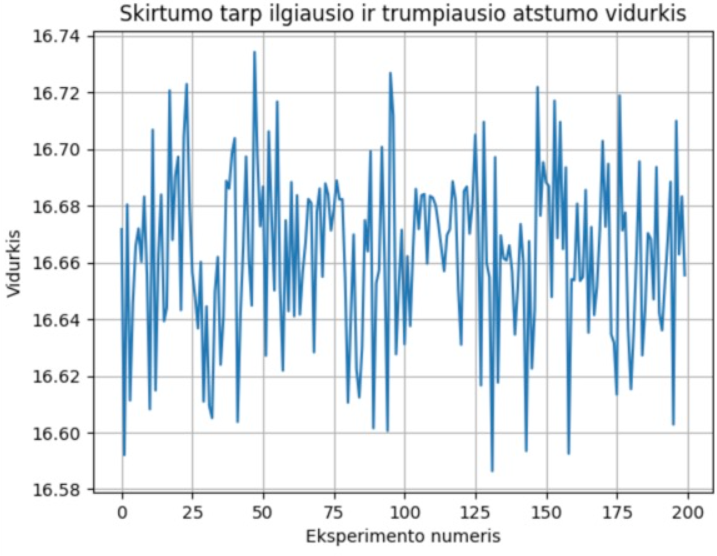
\includegraphics[scale = .53]{skirtumo_vidurkis_k3.png}
    \caption{viršūnės kaimynių skaičius = 3}
  \label{fig:vidurkis_k3}
\end{subfigure}%
\begin{subfigure}{.5\textwidth}
  \centering
  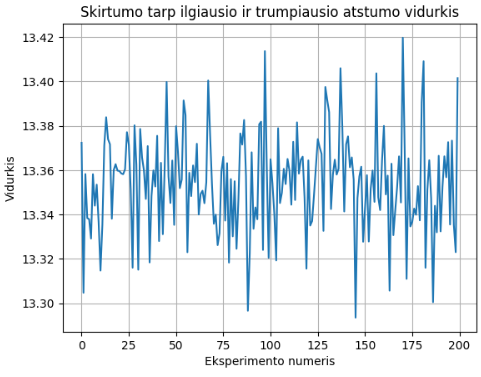
\includegraphics[scale = .8]{skirtumo_vidurkis_k4.png}
    \caption{viršūnės kaimynių skaičius = 4}
  \label{fig:vidurkis_k4}
\end{subfigure}
\caption{}
\end{figure}



Taip pat dar paskaičiavome gautų skirtumų vidurkių (paveikslėliuose \ref{fig:vidurkis_k3} ir \ref{fig:vidurkis_k4}) pasikliovimo intervalus. Naudojome bootstrap funkciją. Kai viršūnių kaimynių skaičius yra 3, tai pasikliovimo apatinis rėžis yra 16,6586, o viršutinis 16,6670. Na, o kai kaimynių skaičius yra 4, tai paskliovimo intervalas yra [13.35123, 13.35732]. 


\begin{figure}[h]
\centering
\begin{subfigure}{.5\textwidth}
  \centering
  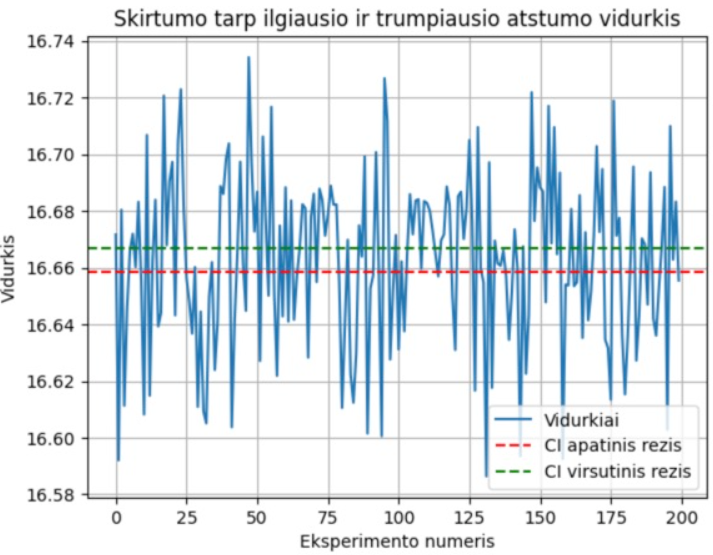
\includegraphics[scale = .53]{CI_k3.png}
    \caption{viršūnės kaimynių skaičius = 3}
  \label{CI_k3}
\end{subfigure}%
\begin{subfigure}{.5\textwidth}
  \centering
  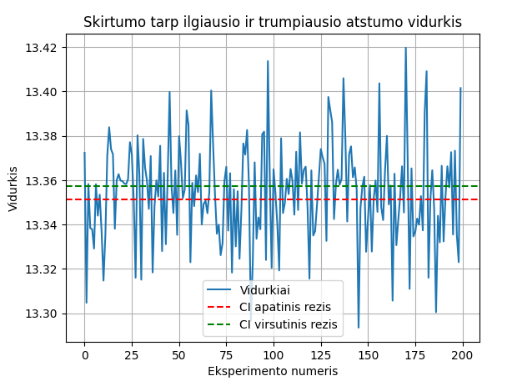
\includegraphics[scale = .8]{CI_k4.png}
    \caption{viršūnės kaimynių skaičius = 4}
  \label{fig:CI_k4}
\end{subfigure}
\caption{}
\end{figure}


\newpage 
\section*{Išvados}
\label{sec:isvados}
\addcontentsline{toc}{section}{\nameref{sec:isvados}}
Atlikus gautų rezultatų analizę, galima padaryti daugiausia trivalias išvadas:



\begin{itemize}
\item Skaičiuodami skirtumą tarp ilgiausio ir trumpiausio atstumo, dažniausiai pasitaikantis skirtumas, kai viršūnės turi po 4 kaimynus, yra 3 vienetais mažesnis nei grafuose, kur viršūnės turi po 3 kaimynus.
\item  Analizuodami didžiausius skirtumus tarp ilgiausio ir trumpiausio atstumo pastebime, kad padidėjus viršūnių kaimynų skaičiui vienetu, dažniausiai pasikartojantis didžiausias skirtumas sumažėja 6 vienetais.
\item Pastebimas skirtumas tarp vidurkio svyravimo diapazonų yra nedidelis, o tyrimo rezultatai patvirtiną spėjimą, kad didelį kaimynių kiekį turinti viršūnė įtakos mažesnio skirtumo rezultatą tarp ilgiausio ir trumpiausio kelio.




\end{itemize}





\newpage 

%\bibliographystyle{unsrt}

%\bibliography{reference}

\begin{thebibliography}{}

 \bibitem{Floyd-Warshall algoritmas}
        Wikipedia
        \newblock \emph{Floyd-Warshall algorithm}
        \newblock \url{https://en.wikipedia.org/wiki/Floyd-Warshall_algorithm}

\bibitem{Floyd-Warshall algoritmas}
        Programiz.com
        \newblock \emph{Floyd-Warshall algorithm}
        \newblock \url{https://www.programiz.com/dsa/floyd-warshall-algorithm}

\bibitem{Floyd-Warshall algoritmas sprendžiant trumpiausių kelių problemą}
    ICASI 2018
    \newblock \emph{Floyd-Warshall algorithm in shortest path problem}
        \newblock \url{https://books.google.lt/books?hl=lt&lr=&id=MDBdEAAAQBAJ&oi=fnd&pg=PA47&dq=Search+for+connected+components+in+a+direct+graph+floyd+warshall&ots=I6YerbMVn3&sig=ZqSXvl_7DE2dbCMQBMw1aN4VnL8&redir_esc=y#v=onepage&q&f=false}
\end{thebibliography}



\newpage 
\appendix
\section*{Priedai. Kodas}

Tyrimo kodas Collab aplinkoje:

\url{https://colab.research.google.com/drive/1nkvBS-fKhPbs9gpjYyCdsVGuO-59Rf4L?usp=sharing}


\end{document}

